\clearpage
\section{Results of simulation study to assess the performance of estimators}\label{Results}

The performance of the estimators is assessed using simulation studies as described in chapter~\ref{Simulation}. A good estimator has high precision (small width of confidence interval) and good coverage probability.

A guide to the labels for estimators in graphs and tables:
\begin{itemize}
	\item SRS: Simple Random Sample estimator (section~\ref{SRS})
	\item Bootstrap SRS: simple Random Sample with Bootstrap (section~\ref{SRSBoot})
	\item Cochran 1977: Linear regression estimator (section~\ref{AuxCochran})
	\item van Zanten: van Zanten estimator (section~\ref{AuxVZ})
	\item Bootstrap regression: Linear regression estimator with Bootstrap (section~\ref{AuxBoot})
\end{itemize}

Estimators that do not rely on the bootstrap are computationally inexpensive, and can be applied quickly to a large number of synthetic data sets. This allows us to assess the coverage probability (a large number of trials is needed to get a reliable estimate) for a variety of scenarios. There are many scenarios that can be explored, and the web-App can be a suitable tool to do this. A number of scenarios are illustrated here. For each scenario, results are generated for a range of sample sizes and a range of correlations between auxiliary variable and EF. For all scenarios, the average EF and variability in EF are similar to that observed in the Pernis data ($\mu_y=1.5$ and $\sigma_y=0.1$; see chapter~\ref{Pernis}). For each scenario, the results are based on 2500 synthetic data sets: 
\begin{itemize}
	\item ``High variability in flow rates; no correlation between EF and flow rates'': figure~\ref{fig:Batch3}.
	\item ``Low variability in flow rates; no correlation between EF and flow rates'': figure~\ref{fig:Batch4}.
	\item ``High variability in flow rates; correlation between EF and flow rates'': figure~\ref{fig:Batch5}.
\end{itemize}

In all cases, the use of an auxiliary variable greatly improves the precision of the estimate of the annual average EF. The stronger the correlation between EF and auxiliary variable, the greater the increase in precision. As expected, precision increases as a function of sample size $n$. Increasing the variability in flow rate does not have a large impact on the precision of the estimate (compare figure~\ref{fig:Batch3} with figure~\ref{fig:Batch4}), but the coverage probability of the Cochran 1977 estimator is somewhat too low when the flow rates are highly variable. When the flow rate is correlated with the EF, the coverage probability of the Cochran 1977 estimator is somewhat too low, but the coverage probability of the van Zanten estimator is much too low (figure~\ref{fig:Batch5}). The standard of 0.5\% relative uncertainty can only be met with a combination of very strong correlation between auxiliary variable and large sample size. 

\begin{figure}[h]
	\centering
	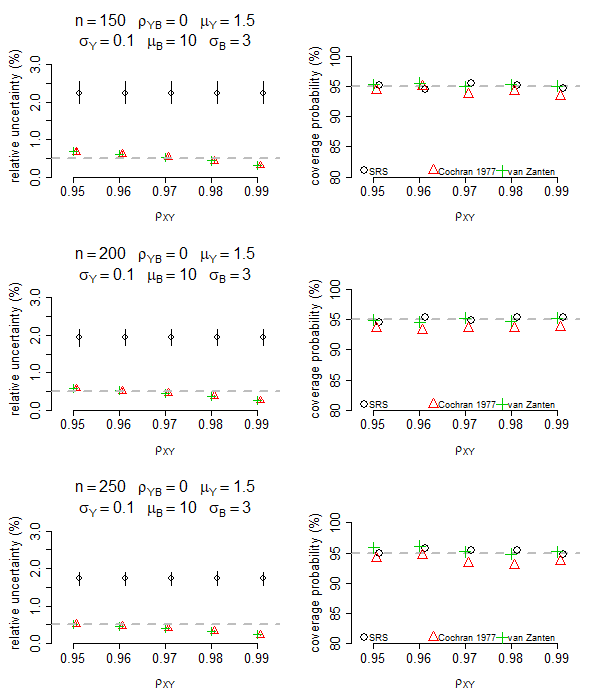
\includegraphics[width=\textwidth]{graphs/Results_Combined_withoutBoot_200.png}
	\caption{Relative uncertainty of the mean annual EF estimate, and coverage probability of the 95\% confidence interval, for the SRS, van Zanten and Cochran 1977 estimators. Scenario: no correlation between auxiliary variable and EF ($\rho_{YB}=0$), high variability in flow rates ($\mu_B=10$, $\sigma_B=3$). }
	\label{fig:Batch3}
\end{figure}

\begin{figure}[h]
	\centering
	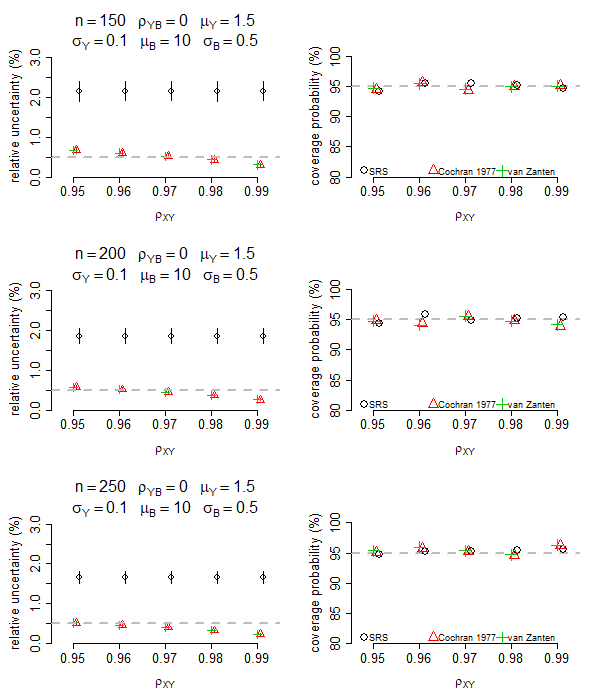
\includegraphics[width=\textwidth]{graphs/Results_Combined_withoutBoot_LowFlowRateVar250.png}
	\caption{Relative uncertainty of the mean annual EF estimate, and coverage probability of the 95\% confidence interval, for the SRS, van Zanten and Cochran 1977 estimators. Scenario: no correlation between auxiliary variable and EF ($\rho_{YB}=0$), low variability in flow rates ($\mu_B=10$, $\sigma_B=0.5$), no correlation between flow rate and EF ($\rho_{YB}$).}
	\label{fig:Batch4}
\end{figure}

\begin{figure}[h]
	\centering
	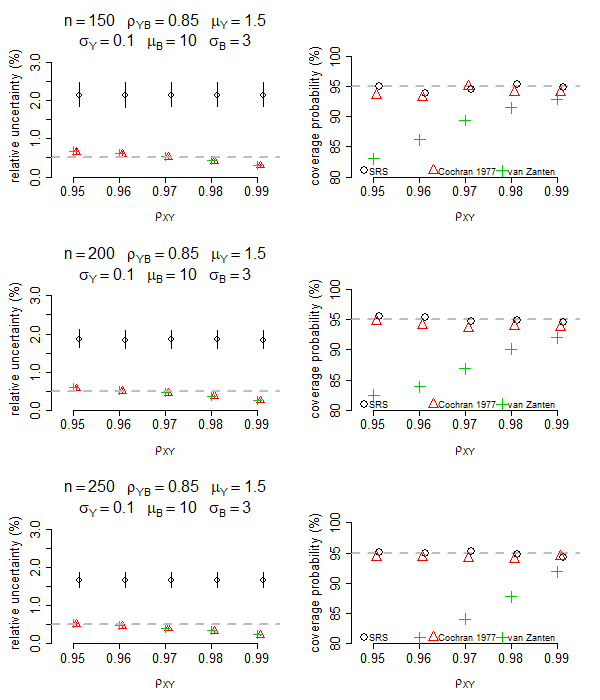
\includegraphics[width=\textwidth]{graphs/Results_Combined_withoutBoot_HighFlowRateVar_corB250.png}
	\caption{Relative uncertainty of the mean annual EF estimate, and coverage probability of the 95\% confidence interval, for the SRS, van Zanten and Cochran 1977 estimators. Scenario: strong correlation between auxiliary variable and EF ($\rho_{YB}=0.85$), high variability in flow rates ($\mu_B=10$, $\sigma_B=3$).}
	\label{fig:Batch5}
\end{figure}

The Bootstrap estimators are computationally intensive (see chapter~\ref{Estimators}), and a smaller number of  scenarios has been included for illustration here. For each scenario, the results are based on 2500 synthetic data sets: 
\begin{itemize}
	%\item Average and variability in EF similar to that observed in the Pernis fuel gas ($\mu_Y=1.5$, $\sigma_Y=0.1$), some variability in flow rates ($\mu_B=10$, $\sigma_B=1$), strong correlation between auxiliary variable and EF ($\rho_{YX}=0.96$) and no correlation between flow rate and EF ($\rho_{YB}=0$): table~\ref{tab:batch1}.
	\item Variability in EF similar to that observed in the Pernis fuel gas ($\mu_Y=1.5$, $\sigma_Y=0.1$), very high variability in flow rates ($\mu_B=10$, $\sigma_B=3$), strong correlation between auxiliary variable and EF ($\rho_{YX}=0.96$) and no correlation between flow rate and EF ($\rho_{YB}=0$): table~\ref{tab:batch2}.
	\item Variability in EF similar to that observed in the Pernis fuel gas ($\mu_Y=1.5$, $\sigma_Y=0.1$), very high variability in flow rates ($\mu_B=10$, $\sigma_B=3$), strong correlation between auxiliary variable and EF ($\rho_{YX}=0.96$) and strong correlation between flow rate and EF ($\rho_{YB}=0.85$): table~\ref{tab:batch3}.
	\item Variability in EF similar to that observed in the Pernis fuel gas ($\mu_Y=1.5$, $\sigma_Y=0.1$), low variability in flow rates ($\mu_B=10$, $\sigma_B=0.5$), very strong correlation between auxiliary variable and EF ($\rho_{YX}=0.99$) and no correlation between flow rate and EF ($\rho_{YB}=0.85$): table~\ref{tab:batch4}.
	\item Higher variability in EF similar compared to that observed in the Pernis fuel gas ($\mu_Y=1.5$, $\sigma_Y=0.15$), low variability in flow rates ($\mu_B=10$, $\sigma_B=0.5$), very strong correlation between auxiliary variable and EF ($\rho_{YX}=0.99$) and no correlation between flow rate and EF ($\rho_{YB}=0.85$): table~\ref{tab:batch5}.
\end{itemize}

The Bootstrap estimators yield very similar estimates of relative uncertainty compared to their analytical counterparts (compare SRS with Bootstrap SRS, and van Zanten or Cochran 1977 with Boostrap regression). When flow rate and EF are correlated, the van Zanten estimator has suboptimal coverage probability but the Bootstrap regression estimator performs well (table~\ref{tab:batch3} and ~\ref{tab:batch5}). The relative uncertainty is very low when the sample size is $n=200$ and when there is strong correlation between auxliary variable and EF ($\rho_{XY}=0.99$; table~\ref{tab:batch4}). the relative uncertainty increases substantially when the variability in EF increases (table~\ref{tab:batch5}).

%\begin{table}
%	\caption{Performance of estimators in a scenario with average and variability in EF similar to that observed in the Pernis fuel gas ($\mu_Y=1.5$, $\sigma_Y=0.1$),some variability in flow rates ($\mu_B=10$, $\sigma_B=1$), strong correlation between auxiliary variable and EF ($\rho_{YX}=0.96$) and no correlation between flow rate and EF ($\rho_{YB}=0$). }
%	\begin{tabular}{l l r@{.}l@{ - }r@{.}l r@{.}l@{ - }r@{.}l}
%		\hline
%		$n$ & Estimator & \multicolumn{4}{c}{Relative Uncertainty (\%)} & \multicolumn{4}{c}{Coverage probability (\%)} \\
%		\hline
%		100 & SRS 		 		& 2&30&3&01 & 93&01&95&83 \\
%		    & Bootstrap SRS 	& 2&23&2&99 & 92&87&95&65 \\
%		    & van Zanten   		& 0&64&0&85 & 94&25&96&78 \\
%		    & Cochran 1977 		& 0&64&0&84 & 93&97&96&52 \\
%		    & Boostrap regression & 0&62&0&85 & 93&79&96&44 \\
%		\cline{2-10}
%		200 & SRS 		 		& 1&64&2&05 & 93&23&96&00 \\
%		    & Bootstrap SRS 	& 1&65&2&06 & 93&01&95&83 \\
%		    & van Zanten   		& 0&47&0&58 & 94&70&97&12 \\
%		    & Cochran 1977 		& 0&47&0&57 & 94&59&97&04 \\
%		    & Boostrap regression & 0&46&0&58 & 94&59&97&04 \\
%		\hline
%	\end{tabular} \label{tab:batch1}
%\end{table}


\begin{table}
	\caption{Performance of estimators in a scenario with average and variability in EF similar to that observed in the Pernis fuel gas ($\mu_Y=1.5$, $\sigma_Y=0.1$), very high variability in flow rates ($\mu_B=10$, $\sigma_B=3$), strong correlation between auxiliary variable and EF ($\rho_{YX}=0.96$) and no correlation between flow rate and EF ($\rho_{YB}=0$).}
	\begin{tabular}{l l r@{.}l@{ - }r@{.}l r@{.}l@{ - }r@{.}l}
		\hline
		$n$ & Estimator & \multicolumn{4}{c}{Relative Uncertainty (\%)} & \multicolumn{4}{c}{Coverage probability (\%)} \\
		\hline
		100 & SRS 		 		& 2&33&3&26 & 94&02&96&61 \\
		    & Bootstrap SRS 	& 2&25&3&18 & 93&45&96&18 \\
		    & van Zanten   		& 0&64&0&85 & 93&45&96&18 \\
		    & Cochran 1977 		& 0&64&0&84 & 92&67&95&56 \\
		    & Boostrap regression & 0&62&0&85 & 92&45&95&39 \\
		\cline{2-10}
		200 & SRS 		 		& 1&73&2&05 & 93&79&96&44 \\
		    & Bootstrap SRS 	& 1&67&2&06 & 93&68&96&35 \\
		    & van Zanten   		& 0&47&0&58 & 95&05&97&38 \\
		    & Cochran 1977 		& 0&47&0&57 & 93&34&96&09 \\
		    & Boostrap regression & 0&46&0&58 & 94&25&96&78 \\
		\hline
	\end{tabular}\label{tab:batch2}
\end{table}

\begin{table}
	\caption{Performance of estimators in a scenario with average and variability in EF similar to that observed in the Pernis fuel gas ($\mu_Y=1.5$, $\sigma_Y=0.1$), very high variability in flow rates ($\mu_B=10$, $\sigma_B=3$), strong correlation between auxiliary variable and EF ($\rho_{YX}=0.96$) and strong correlation between flow rate and EF ($\rho_{YB}=0.85$).}
	\begin{tabular}{l l r@{.}l@{ - }r@{.}l r@{.}l@{ - }r@{.}l}
		\hline
		$n$ & Estimator & \multicolumn{4}{c}{Relative Uncertainty (\%)} & \multicolumn{4}{c}{Coverage probability (\%)} \\
		\hline 
		100 & SRS 		 		& 2&20&3&17 & 93&57&96&26 \\
		    & Bootstrap SRS 	& 2&13&3&15 & 93&12&95&91 \\
		    & van Zanten   		& 0&65&0&87 & 88&39&92&06 \\
		    & Cochran 1977 		& 0&63&0&83 & 92&34&95&30 \\
		    & Boostrap regression & 0&57&0&83 & 92&54&95&39 \\
		\cline{2-10}
		200 & SRS 		 		& 1&61&2&11 & 93&12&95&92 \\
		    & Bootstrap SRS 	& 1&56&2&10 & 92&23&95&21 \\
		    & van Zanten   		& 0&48&0&59 & 81&24&85&83 \\
		    & Cochran 1977 		& 0&46&0&56 & 92&89&95&74 \\
		    & Boostrap regression & 0&42&0&55 & 93&57&96&26 \\
		\hline
	\end{tabular}\label{tab:batch3}
\end{table}


\begin{table}
	\caption{Performance of estimators in a scenario with average and variability in EF similar to that observed in the Pernis fuel gas ($\mu_Y=1.5$, $\sigma_Y=0.1$), low variability in flow rates ($\mu_B=10$, $\sigma_B=0.5$), very strong correlation between auxiliary variable and EF ($\rho_{YX}=0.99$) and no correlation between flow rate and EF ($\rho_{YB}=0.85$).}
	\begin{tabular}{l l r@{.}l@{ - }r@{.}l r@{.}l@{ - }r@{.}l}
		\hline
		$n$ & Estimator & \multicolumn{4}{c}{Relative Uncertainty (\%)} & \multicolumn{4}{c}{Coverage probability (\%)} \\
		\hline
		100 & SRS 		 		& 2&28&3&01 & 93&01&95&83 \\
		    & Bootstrap SRS 	& 2&20&2&98 & 92&34&95&30 \\
		    & van Zanten   		& 0&32&0&43 & 94&25&96&78 \\
		    & Cochran 1977 		& 0&32&0&43 & 94&47&96&95 \\
		    & Boostrap regression & 0&31&0&43 & 94&25&96&30 \\
		\cline{2-10}
		200 & SRS 		 		& 1&68&2&05 & 93&91&96&52 \\
		    & Bootstrap SRS 	& 1&63&2&05 & 92&12&95&91 \\
		    & van Zanten   		& 0&24&0&29 & 93&79&96&44 \\
		    & Cochran 1977 		& 0&24&0&29 & 93&68&96&35 \\
		    & Boostrap regression & 0&23&0&29 & 93&57&96&26 \\
		\hline
	\end{tabular}\label{tab:batch4}
\end{table}


\begin{table}
	\caption{Performance of estimators in a scenario with higher variability in EF similar compared to that observed in the Pernis fuel gas ($\mu_Y=1.5$, $\sigma_Y=0.15$), low variability in flow rates ($\mu_B=10$, $\sigma_B=0.5$), very strong correlation between auxiliary variable and EF ($\rho_{YX}=0.99$) and no correlation between flow rate and EF ($\rho_{YB}=0.85$).}
	\begin{tabular}{l l r@{.}l@{ - }r@{.}l r@{.}l@{ - }r@{.}l}
		\hline
		$n$ & Estimator & \multicolumn{4}{c}{Relative Uncertainty (\%)} & \multicolumn{4}{c}{Coverage probability (\%)} \\
		\hline
		100 & SRS 		 		& 3&38&4&52 & 92&67&95&56 \\
		    & Bootstrap SRS 	& 3&72&4&46 & 91&67&94&76 \\
		    & van Zanten   		& 0&49&0&65 & 92&00&95&03 \\
		    & Cochran 1977 		& 0&49&0&65 & 91&34&94&50 \\
	        & Boostrap regression & 0&47&0&65 & 92&00&95&03 \\
		\cline{2-10}
		200 & SRS 		 		& 2&52&3&07 & 94&13&96&70 \\
		    & Bootstrap SRS 	& 2&45&3&06 & 93&97&96&52 \\
		    & van Zanten   		& 0&36&0&44 & 93&45&96&18 \\
		    & Cochran 1977 		& 0&35&0&43 & 93&01&95&83 \\
		    & Boostrap regression & 0&35&0&44 & 92&78&95&65 \\
		\hline
	\end{tabular}\label{tab:batch5}
\end{table}




%\begin{table}
%	\caption{Scenario 1: $\mu_Y=1.5$, $\sigma_Y=0.1$, $\mu_B=10$, $\sigma_B=1$, $\rho_{YX}=0.96$, $\rho_{YB}=0$. Scenario 2: $\mu_Y=1.5$, $\sigma_Y=0.1$, $\mu_B=10$, $\sigma_B=3$, $\rho_{YX}=0.96$, $\rho_{YB}=0$. Scenario 3: $\mu_Y=1.5$, $\sigma_Y=0.1$, $\mu_B=10$, $\sigma_B=3$, $\rho_{YX}=0.96$, $\rho_{YB}=0.85$. Scenario 4: $\mu_Y=1.5$, $\sigma_Y=0.1$, $\mu_B=10$, $\sigma_B=0.5$, $\rho_{YX}=0.99$, $\rho_{YB}=0$. Scenario 5: $\mu_Y=1.5$, $\sigma_Y=0.15$, $\mu_B=10$, $\sigma_B=0.5$, $\rho_{YX}=0.99$, $\rho_{YB}=0$.}
%	\begin{tabular}{l l l r@{.}l@{ - }r@{.}l r@{.}l@{ - }r@{.}l}
%		\hline \hline
%		Scenario & $n$ & Estimator & \multicolumn{4}{c}{Relative Uncertainty (\%)} & \multicolumn{4}{c}{Coverage probability (\%)} \\
%		\hline
%		1   & 100 & SRS 		 		& 2&30&3&01 & 93&01&95&83 \\
%		& 	  & Bootstrap SRS 		& 2&23&2&99 & 92&87&95&65 \\
%		& 	  & van Zanten   		& 0&64&0&85 & 94&25&96&78 \\
%		&     & Cochran 1977 		& 0&64&0&84 & 93&97&96&52 \\
%		&	  & Boostrap regression & 0&62&0&85 & 93&79&96&44 \\
%		\cline{2-11}
%		& 200 & SRS 		 		& 1&64&2&05 & 93&23&96&00 \\
%		& 	  & Bootstrap SRS 		& 1&65&2&06 & 93&01&95&83 \\
%		& 	  & van Zanten   		& 0&47&0&58 & 94&70&97&12 \\
%		&     & Cochran 1977 		& 0&47&0&57 & 94&59&97&04 \\
%		&	  & Boostrap regression & 0&46&0&58 & 94&59&97&04 \\
%		\hline 
%		2   & 100 & SRS 		 		& 2&33&3&26 & 94&02&96&61 \\
%		& 	  & Bootstrap SRS 		& 2&25&3&18 & 93&45&96&18 \\
%		& 	  & van Zanten   		& 0&64&0&85 & 93&45&96&18 \\
%		&     & Cochran 1977 		& 0&64&0&84 & 92&67&95&56 \\
%		&	  & Boostrap regression & 0&62&0&85 & 92&45&95&39 \\
%		\cline{2-11}
%		& 200 & SRS 		 		& 1&73&2&05 & 93&79&96&44 \\
%		& 	  & Bootstrap SRS 		& 1&67&2&06 & 93&68&96&35 \\
%		& 	  & van Zanten   		& 0&47&0&58 & 95&05&97&38 \\
%		&     & Cochran 1977 		& 0&47&0&57 & 93&34&96&09 \\
%		&	  & Boostrap regression & 0&46&0&58 & 94&25&96&78 \\
%		\hline 
%		3   & 100 & SRS 		 		& 2&20&3&17 & 93&57&96&26 \\
%		& 	  & Bootstrap SRS 		& 2&13&3&15 & 93&12&95&91 \\
%		& 	  & van Zanten   		& 0&65&0&87 & 88&39&92&06 \\
%		&     & Cochran 1977 		& 0&63&0&83 & 92&34&95&30 \\
%		&	  & Boostrap regression & 0&57&0&83 & 92&54&95&39 \\
%		\cline{2-11}
%		& 200 & SRS 		 		& 1&61&2&11 & 93&12&95&92 \\
%		& 	  & Bootstrap SRS 		& 1&56&2&10 & 92&23&95&21 \\
%		& 	  & van Zanten   		& 0&48&0&59 & 81&24&85&83 \\
%		&     & Cochran 1977 		& 0&46&0&56 & 92&89&95&74 \\
%		&	  & Boostrap regression & 0&42&0&55 & 93&57&96&26 \\
%		\hline 
%		4   & 100 & SRS 		 		& 2&28&3&01 & 93&01&95&83 \\
%		& 	  & Bootstrap SRS 		& 2&20&2&98 & 92&34&95&30 \\
%		& 	  & van Zanten   		& 0&32&0&43 & 94&25&96&78 \\
%		&     & Cochran 1977 		& 0&32&0&43 & 94&47&96&95 \\
%		&	  & Boostrap regression & 0&31&0&43 & 94&25&96&30 \\
%		\cline{2-11}
%		& 200 & SRS 		 		& 1&68&2&05 & 93&91&96&52 \\
%		& 	  & Bootstrap SRS 		& 1&63&2&05 & 92&12&95&91 \\
%		& 	  & van Zanten   		& 0&24&0&29 & 93&79&96&44 \\
%		&     & Cochran 1977 		& 0&24&0&29 & 93&68&96&35 \\
%		&	  & Boostrap regression & 0&23&0&29 & 93&57&96&26 \\
%		\hline 
%		5   & 100 & SRS 		 		& 3&38&4&52 & 92&67&95&56 \\
%		& 	  & Bootstrap SRS 		& 3&72&4&46 & 91&67&94&76 \\
%		& 	  & van Zanten   		& 0&49&0&65 & 92&00&95&03 \\
%		&     & Cochran 1977 		& 0&49&0&65 & 91&34&94&50 \\
%		&	  & Boostrap regression & 0&47&0&65 & 92&00&95&03 \\
%		\cline{2-11}
%		& 200 & SRS 		 		& 2&52&3&07 & 94&13&96&70 \\
%		& 	  & Bootstrap SRS 		& 2&45&3&06 & 93&97&96&52 \\
%		& 	  & van Zanten   		& 0&36&0&44 & 93&45&96&18 \\
%		&     & Cochran 1977 		& 0&35&0&43 & 93&01&95&83 \\
%		&	  & Boostrap regression & 0&35&0&44 & 92&78&95&65 \\
%		\hline 	\hline
%	\end{tabular}
%\end{table}